%A classe é a dcc-nce, e o parâmetro a ser informado é diss (para dissertação de mestrado)
\documentclass[diss]{dcc-nce}
\usepackage[T1]{fontenc}
\usepackage{color,graphicx}
\usepackage{graphics}
\usepackage{url}
\usepackage{amsmath,amssymb}
%\usepackage[numbers]{natbib}
\usepackage{natbib}
\usepackage{dsfont} %Usado para conjuntos N, Z, Q, R, C
\usepackage[portugues,algoruled,longend]{algorithm2e}
\usepackage{algorithmic}
\usepackage[utf8]{inputenc}
\usepackage{listings}%Para inserir codigos fontes de programas no apendice.
\usepackage{xcolor}
% Definindo novas cores
\definecolor{verde}{rgb}{0,0.5,0}
% Configurando layout para mostrar codigos C++
\usepackage{listings}
\lstset{
  language=C++,
  basicstyle=\ttfamily\small,
  keywordstyle=\color{blue},
  stringstyle=\color{verde},
  commentstyle=\color{red},
  extendedchars=true,
  showspaces=false,
  showstringspaces=false,
  numbers=left,
  numberstyle=\tiny,
  breaklines=true,
  backgroundcolor=\color{green!10},
  breakautoindent=true,
  captionpos=b,
  xleftmargin=0pt,
}


\topmargin=0in
\textheight=20.5cm


\begin{document}

%Este tem que vir primeiro neste arquivo, caso contrario nao aparecerao
%as palavras-chave na ficha catalografica:
\keyword{Casos de teste}
\keyword{UML - Unified Modeling Language}
\keyword{OCL - Object Constaint Language}

\cip{}


    % Editar o arquivo palavrasChavePortugues

%O restante vem depois:
\title{Uma Abordagem para Geração Automática de Casos de Teste Independentes de Plataforma Utilizando UML e OCL}

% COLOCAR AQUI O CUTTER (CÓDIGO FORNECIDO PELA BIBLIOTECA DO NCE PARA A FICHA CATALOGRÁFICA):
\codigobiblioteca{CBIB}

\author{Dias}{Marcos Vinicius Furriel Amorim Dias}
\advisor[Dr.]{Schmitz}{Eber Assis Schmitz}
\coadvisor[Profa. Dra.]{Último Sobrenome}{Nome Sobrenome1 Sobrenome2 ...}
\banca{Profa. Dr. Fulano de Tal}{Prof. Dr. Beltrano}{Prof. Dr. Ciclano}
\date{2016}
\maketitle
                      % Editar o arquivo capa.tex
\clearpage

\mbox{}\vfill

\begin{flushright}

{\sffamily\itshape

Aqui coloque a dedicatória...

Se não houver, delete esta parte.

}

\end{flushright}
               % Editar o arquivo dedicatoria.tex
\begin{agradecimentos}
Coloque aqui os agradecimentos.

Agradeço aos meus pais, meu orientador, à bolsa, etc...
\end{agradecimentos}
            % Editar o arquivo agradecimentos.tex
\begin{abstract}

%MADUREIRA, Rodrigo Lopes Rangel. Algoritmos de interseções, bla bla bla...\\

FURRIEL, Marcos Vinicius. Uma Abordagem para Geração Automática de Casos de Teste Independentes de Plataforma utilizando UML/OCL. 2015. x f. Dissertação (Mestrado em Informática) – Instituto de Matemática e Instituto Tércio Pacitti de Aplicações e Pesquisas Computacionais, Universidade Federal do Rio de Janeiro, Rio de Janeiro, 2016.


Esta dissertação apresentará um protótipo ferramental utilizando a abordagem MDA para geração  de  casos  de  teste  independentes  de  plataforma  a  partir  de  diagramas  de  classe enriquecidos com anotações OCL. Além disso, também é apresentada uma fundamentação teórica sobre conceitos de Teste de Software e da Engenharia Orientada a Modelos, bem como as transformações da MDA e suas principais características.


\end{abstract}
           % Editar o arquivo resumoPortugues.tex
%\begin{englishabstract}{Colocar aqui o título da dissertação em inglês}{coloque aqui as palavras-chave em inglês, separadas por vírgula}

\begin{englishabstract}{}{coloque aqui as palavras-chave em inglês, separadas por vírgula}


%MADUREIRA, Rodrigo Lopes Rangel. Algoritmos de interseções, bla bla bla...\\

Colocar aqui o resumo em inglês.
\end{englishabstract}

              % Editar o arquivo resumoIngles.tex

\listoffigures{}

\listoftables{}

%% Examples

\begin{listofabbrv}{XXXXXX}
  \item [BCNF] Boyce Codd Normal Form
  \item [XSLT] XSL Transformations
\end{listofabbrv}
    % Editar o arquivo listaAbreviaturaSiglas.tex

\tableofcontents{}                  % Sumário

\parindent=1.25cm %start for each paragraph from the left margin
\parskip=20pt
\baselineskip=20pt


\chapter{Introdução}

Este capítulo está dividido em quatro seções. A seção 1.1 apresenta a motivação para realização deste trabalho. A seção 1.2 descreve o problema a ser tratado nesta dissertação. A seção 1.3 mostra as questões que nortearam esta pesquisa. A seção 1.4 os objetivos e o escopo deste trabalho. Por fim, a seção 1.5 descreve a estrutura segundo a qual este trabalho está organizado.

%Este é um relatório técnico \cite{BON03}, um livro \cite{SILBERSCHATZ}, um relatório técnico \cite{PIERCE}, referência da Web \cite{DB2XML}, trabalho de final de curso \cite{Angelo}, e tese de doutorado \cite{HAR98}.

%Artigo sem ano \citet{SPH03}.
%Artigo sem ano \citet{SPH03}.  \\
Artigo sem ano \citet{Longuet-1950}.   \\
%\citet{Hou95} \\
%\citeauthor{Hou95} \\
%\citeonline{Hou95}
Em \citep{SPH_LIU_2003}
Em \cite{Scan-1990-Blelloch}

\section{Motivação}

%Uma seção...

%Agora vamos referenciar a Figura \ref{figuraEPS}.

A criação manual de Casos de Teste por vezes é muito trabalhosa, sendo uma tarefa que compromete tempo e recursos por parte dos Analistas de Teste (SOUSA, 2009). Além disso, o trabalho de criação manual dos casos de teste pode ser considerado uma tarefa entediante (ISMAIL, 2007), o que pode afetar a forma como os testes são planejados e construídos. Dessa forma o analista de teste pode não alcançar uma cobertura de restrições positivas e negativas satisfatórias prejudicando a qualidade esperada para o software (SILVA-DE-SOUZA, 2012).

Com o passar dos anos a preocupação com relação à qualidade do software aumenta consideravelmente a medida que a complexidade dos sistemas evolui (SILVA-DE-SOUZA, 2012). Ao escolher uma abordagem orientada a Modelos uma parte desta complexidade é abstraída do desenvolvimento e o analista passa a ter a chance de criar os seus modelos de teste independentemente da plataforma utilizada, gerando maior portabilidade entre os sistemas da informação (BRAMBILLA, CABOT E WIMMER, 2012). A possibilidade de automatizar a criação de variados procedimentos de testes a partir de um simples modelo em alto nível de abstração torna o desenvolvimento mais veloz, menos dependente de tecnologia e sem necessidade de conhecimento profundo em determinada linguagem de programação, diminuindo a quantidade de recursos superutilizados, tempo, custo e aos riscos aos quais o desenvolvimento está sujeito (SOUSA, 2009). Ao possibilitar que a criação dos casos de teste seja realizada de forma automática diretamente a partir de diagramas de classe que expressem o domínio e suas regras de negócio, pode-se então diminuir o tempo e os recursos gastos durante o desenvolvimento.

\section{Problemática}

Segundo Sousa (2009) os maiores esforços durante o ciclo de desenvolvimento de um software se concentram na fase de teste, que chegam a atingir cerca de 50 /percent ou mais dos custos de desenvolvimento de software (XU et al, 2015). Nesta fase é notado um grande desperdício de tempo, custo e recursos por parte das desenvolvedoras. Além disso, a construção manual dos casos de teste acaba por generalizar eventuais erros humanos, abrindo possibilidade para que defeitos se propaguem durante todo o desenvolvimento afetando diretamente a qualidade do produto final (SOUSA, 2009).

\section{Objetivo do Trabalho}

O objetivo geral deste trabalho é definir uma abordagem que possibilite a geração automática de casos de teste para independentes de plataforma a partir de modelos de classes UML enriquecidos com restrições OCL.

\section{Organização do Trabalho}

Esta dissertação está organizada em sete capítulos. O capítulo 1 mostrou a introdução do trabalho, ressaltando a sua motivação, o problema tratado e seus objetivos. O capítulo 2 discorre sobre o referencial teórico deste trabalho, através de um resumo da revisão bibliográfica. O capítulo 3 apresenta a abordagem proposta, através de um exemplo simples. O capítulo 4 descreve a metodologia aplicada para colher indícios da utilidade da abordagem proposta e responder as perguntas da pesquisa. O capítulo 5 apresenta os resultados obtidos após a utilização da metodologia, e por fim o capitulo 6 conclui a dissertação, apresentando as considerações finais, contribuições e sugestões de trabalhos futuros. Em seguida, é apresentada a lista de referências bibliográficas utilizadas. Finalmente, são apresentados na forma de apêndices os instrumentos utilizados no estudo quasi-experimental.

%\begin{figure}
   %\begin{center}
     %\scalebox{0.5}{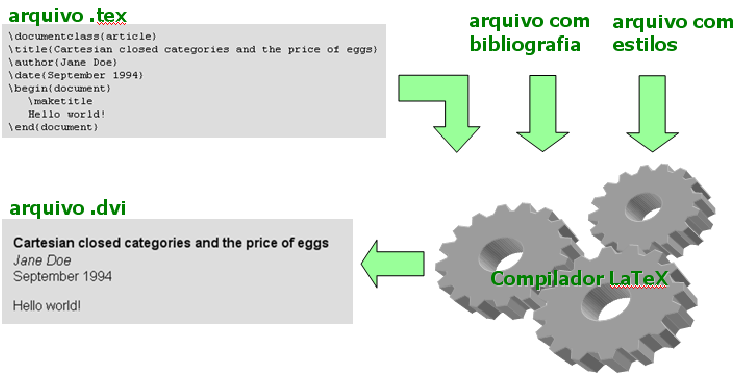
\includegraphics{figs/figuraTeste}}
   %\end{center}
   %\caption{Testando uma figura...\label{figuraEPS}}
%\end{figure}


%\subsection{Bla blá}

%Uma subseção...

%\subsubsection{ABC}

%Uma subsub-seção.
         % Editar o arquivo introducao.tex
\chapter{Referencial Teórico}

Este capítulo trata da fundamentação teórica da dissertação. Ele está dividido em seis seções: a seção 2.1 introduz os conceitos fundamentais sobre Teste de Software; a seção 2.2 descreve os princípios das Regras de Negócio em desenvolvimento de Software; a seção 2.3 apresenta aspectos sobre a linguagem OCL, utilizada para descrever restrições sobre modelos UML; a seção 2.4 apresenta conceitos a respeito da Arquitetura Orientada a Modelos; a seção 2.5 enfatiza o plugin para transformação entre modelos ATL e por fim a seção 2.6 apresenta os trabalhos relacionados a esta pesquisa.

\section{Teste de Software}


Um teste de software consiste na execução de programas onde se tem um valor de entrada, e este por sua vez resultará em uma determinada saída, que será avaliada em função dos resultados esperados (SILVA-DE-SOUZA, 2012). O teste de software tem por objetivo garantir qualidade tanto do produto final quanto de seu desenvolvimento (SILVA-DE-SOUZA, 2012). Segundo Delamaro, Maldonado e Jino (2007) essa garantia de qualidade é conseguida através de processos de Verificação e Validação do Software. Enquanto a primeira tem por objetivo avaliar o software quanto a sua especificação documentada, a segunda objetiva avalia-lo tendo como partida o ponto de vista e necessidades do usuário.


Segundo Silva-de-Souza (2012), o processo de verificação é composto por dois tipos de classificações distintas, sendo uma estática e outra dinâmica. Enquanto que verificações estáticas avaliam aspectos documentais do software, verificações dinâmicas atuam sobre o software em tempo de execução. Para Sousa (2009) é fundamental que sejam mantidos testes durante todo o ciclo de vida do software, pois é dessa maneira que falhas e imprevistos são encontrados, aumentando a confiabilidade e qualidade do produto, minimizando eventuais riscos ao qual todo projeto está inerente.


O processo de teste pode ser dividido em três etapas: Preparação do Teste, Execução do Teste e Registro do Teste (IEEE, 1998). Durante a etapa de preparação do teste é observado a fase de planejamento. Nesta fase da preparação do teste são definidas três dimensões que objetivam saber o tipo de teste a ser realizada, a técnica utilizada para efetua-lo e quando realiza-lo (SOUSA, 2009).


Os Tipos de Teste representam o que deve ser testado no sistema, isto é, quais as características do software que serão testadas. Podem ser tanto necessidades funcionais quanto não funcionais. Já as Técnicas de Teste representam como o sistema deverá ser testado e subdivide-se em duas: Caixa Branca e Caixa Preta, a primeira se trata de uma técnica estrutural que leva em conta o código fonte do sistema, ou seja, o analista de teste tem acesso direto ao código, enquanto que a técnica de caixa preta se trata de um teste funcional, onde as verificações e validações são realizadas de acordo com os requisitos do sistema. Em Níveis de Teste é observado o momento no qual o sistema deverá ser testado. As atividades ocorrem em diferentes níveis do desenvolvimento e contém um teste especifico a ser executado (SOMMERVILLE, 2007). A Figura 1 apresenta as dimensões de teste encontradas

//figura aqui

Segundo Silva-de-Souza (2012), através da realização dos testes não é possível dizer que um software está livre de erros, isto é, um teste nunca provará a ausência de defeitos. Para Sousa (2009), defeitos estão ligado ao universo físico e são causados pela interpretação equivoca do desenvolvedor, enquanto que o erro é a manifestação do defeito desenvolvido e falha é o momento no qual o software tem comportamento diferente do esperado por causa de um erro gerado. Entretanto é importante mencionar que mesmo que um software esteja repleto de erros, este poderá nunca vir a apresentar uma falha. A Figura 2 mostra a relação entre Defeito, erro e falha.

//figura aqui

Outro aspecto importante a ser notado segundo Silva-de-Souza (2012) é a inviabilidade de se realizar testes exaustivos, isto é, testar todas as combinações e condições de entrada e saída esperadas. Para contornar esse problema são realizados alguns critérios de teste, onde os principais critérios são (SILVA-DE-SOUZA, 2012) e (TOMMY et al, 2015):

i.	Particionamento em classes de equivalência: É possível reduzir o número de casos de teste , uma vez que esse critério divide os dados de entrada de uma unidade de software em duas classes, onde uma é composta por valores válidos e outra por valores inválidos. 


ii.	Analise do valor Limite: Concentra-se em testes no limite das classes de equivalência, isto é, exploram as fronteiras entre as classes validas e inválidas utilizando valores que estão dentro ou fora dos limites especificados. 


iii.	Grafo de causa-efeito: o teste começa criando um grafo que estabelece a relação entre o efeito(ações esperadas) e suas causas (dados de entrada). 


iv.	Tabela de decisão: casos de teste são projetados para executar combinação de insumos ou causas, sendo mostrado em uma tabela de decisão. 


\section{Regras de Negócio}


As regras de negócio visam controlar os aspectos internos e externos à organização, no que diz respeito a maneira como os negócios são estruturados e operacionalizados (CUNHA, 2009). Segundo (ARAUJO, 2010), regras de negócio definem pré e pós condições as quais devem ser verdadeiras em determinadas situações. Desta maneira, as regras de negócio são parte fundamental do teste em software, tendo em vista que elas definem ou restringem algum ponto de vista do negócio seja no âmbito organizacional ou no âmbito dos Sistema da Informação (CUNHA, 2009). No lado dos Sistemas da Informação, segundo Cunha (2009) as regras de negócio são vistas como uma parte do requisito do sistema, de modo que seja possível projeta-las, implementa-las, testa-las e analisa-las; enquanto que no lado do negócio, as regras são vistas como diretivas responsáveis por conduzir ou influenciar o comportamento do próprio negócio a qual a organização está investindo.


De acordo com Araújo (2010), a execução de um projeto de negócio está diretamente ligada às operações de criação, atualização, recuperação e exclusão dos objetos de negócio. Tais objetos podem ser considerados como instâncias de classes, sejam elas abstratas ou concretas. Dessa maneira, um diagrama de classes da UML pode ser entendido como uma representação dos objetos de negócio, das suas características, bem como suas possíveis restrições e de seus relacionamentos em um modelo independente de plataforma (ARAUJO, 2010). A Figura 3 exemplifica o metamodelo dos diagramas de classes da UML definido pela OMG (2005):

//figura aqui

Como as regras de negócio definem aspectos relacionados às operações CRUD, bem como suas pré e pós condições, é viável que casos de teste possam vir a serem gerados a partir dessas informações. No entanto é necessário que essas informações sejam expressas em linguagem computacional, como a Object Constraint Language (OCL) por exemplo (ARAUJO, 2010) e (SILVA-DE-SOUZA, 2012).

\section{Object Constraint Language}

A OCL (OMG, 2010) é uma linguagem textual de restrição de objetos definida pela OMG cujo objetivo é especificar restrições que não podem ser definidas graficamente em um modelo UML ou aderente ao padrão MOF (SILVA-DE-SOUZA, 2012). Desse modo, a OCL permite um complemento sobre os aspectos de diagramação da UML (ARAUJO, 2010), tais como especificar restrições, especificar pré e pós condições sobre as operações, condições de guarda e regras de derivação, tornar modelos mais condizentes com a realidade e servir como linguagem de consulta (SILVA-DE-SOUZA, 2012).

De acordo com Araújo (2010), cada restrição está associada a um termo do negócio, de modo que suas sentenças estejam divididas em quarto partes: contexto, propriedade, operação e palavras reservadas. A Figura 4 mostra o metamodelo OCL definido pela OMG em 2003.

//figura aqui


Expressões OCL podem resultar em valores simples, objetos, tuplas, ou coleção de valores. Uma coleção pode ser de quarto tipos: Set (Não permite duplicidade dos elementos),

OrderedSet(semelhante ao Set, porém apresenta ordenação dos elementos), Bag( permite duplicidade dos elementos, mas sem ordenação) e Sequence(semelhante ao Bag, porém com ordenação dos valores) (SILVA-DE-SOUZA, 2012).


Através de um conjunto de instruções OCL é possível especificar restrições a respeito da estrutura e do comportamento de um sistema (SILVA-DE-SOUZA, 2012). Tais instruções baseiam primordialmente em contexto que contem invariantes e pré e pós-condições. A Figura 5 apresenta um exemplo simplificado de uma restrição OCL sobre a classe Empregado

//figura aqui

No exemplo acima temos uma classe empregado que possui nome e salário como atributos. A restrição de regra de negócio segundo o OCL expressado como comentário revela que uma instância da classe Empregado não pode ter salário menor do que zero. Além das restrições utilizando invariantes, a OCL como dito anteriormente, permite o uso de pré e pós-condições sobre determinada operação. A Figura 6 apresenta um exemplo simplificado de pré e pós-condições sobre uma operação.

//figura aqui

O uso da OCL no exemplo acima demonstra que para uma Empresa contratar um Empregado é necessário que antes de faça uma pré-condição, que é o fato de o empregado não estar empregado pela empresa, isto é, uma empresa não pode contratar um empregado que já está contratado. Em seguida o uso da palavra reservada post indica uma pós-condição, que garante que após a execução da operação contratar, a instância do empregado foi adicionada ao conjunto de empregados existentes.


Ao permitir que as regras de negócio sejam expressas computacionalmente em um modelo independente de plataforma, a OCL juntamente com a UML possibilita que casos de teste sejam gerados automaticamente (SILVA-DE-SOUZA, 2012). Contudo, para que isso seja possível é necessário que haja uma abordagem que permita a transformação entre diferentes modelos. E é nesse contexto que surge a Model-Driven Architecture (MDA).

\section{Trabalhos Relacionados}

//trabalhos relacionados           % Editar o arquivo capituloA.tex
\chapter{Métodologia Proposta}

O capítulo...
          % Editar o arquivo capituloB.tex
\chapter{Conclusão}

Este trabalho mostrou...

As principais contribuições deste trabalho são...
          % Editar o arquivo introducao.tex

\bibliography{post-text/referencias}          % Editar o arquivo "referencias.bib"
\bibliographystyle{latex-stuff/abnt-ufrgs}      % Procura pelo arquivo "abnt-ufrgs" - normas ABNT.

\clearpage

\appendix
%Obs.: No sistema operacional Windows, ao modificar este arquivo usando WinEdt, pode gerar erro do tipo:

%Error: Unicode char \u8: not set up for use with LaTeX.

%Se esse erro acontecer no WinEdt, modifique o Apêndice no Texmaker, rode nele e depois no WinEdt.


% Se não tiver Apêndice, deixar este arquivo em branco.

\chapter{}

Escrever no Apêndice A

\clearpage

\chapter{}

Escrever no Apêndice B

\clearpage

\chapter{}

Escrever no Apêndice C

(...)
          % Editar o arquivo apendice.tex

\end{document}

%\citep* - citação completa, com todos os autores

%\citeyearpar - cita somente o ano da publicação
